\documentclass[a4paper,11pt]{jsarticle}


% 数式
\usepackage{amsmath,amsfonts}
\usepackage{bm}
\usepackage{physics}
% 画像
\usepackage{graphicx}
\usepackage[dvipdfmx]{color}
% tikz関連
\usepackage{tikz}
\usetikzlibrary{intersections, calc, arrows.meta}
\usepackage{subcaption}


\begin{document}

\title{2次元有限要素法}
\author{伊東秀晃}
\date{\today}
\maketitle

\section{8メッシュ分割}
次の様なメッシュ分割により、2次元有限要素法を実装した。
\begin{figure}
  \centering
  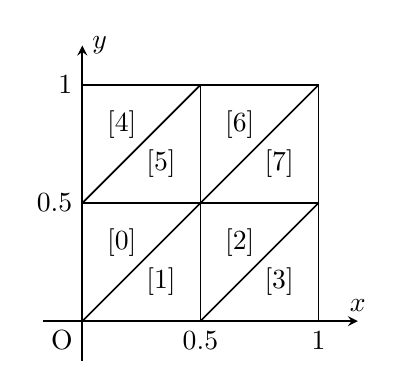
\begin{tikzpicture}
    \draw[->,>=stealth,semithick] (-0.5,0)--(3.5,0)node[above]{$x$}; %x軸
    \draw[->,>=stealth,semithick] (0,-0.5)--(0,3.5)node[right]{$y$}; %y軸
    \draw (0,0)node[below  left]{O}; %原点
    \draw[semithick] (3,0)node[below]{1}--(3,3)--(0,3)node[left]{1}; 
    \draw[semithick] (1.5,0)node[below]{0.5}--(1.5,3); 
    \draw[semithick] (0,1.5)node[left]{0.5}--(3,1.5);
    \draw[semithick] (0,1.5)--(1.5,3);
    \draw[semithick] (0,0)--(3,3);
    \draw[semithick] (1.5,0)--(3,1.5);
    \node at (0.5,1.0) {[0]};
    \node at (1.0,0.5) {[1]};
    \node at (2.0,1.0) {[2]};
    \node at (2.5,0.5) {[3]};
    \node at (0.5,2.5) {[4]};
    \node at (1.0,2.0) {[5]};
    \node at (2.0,2.5) {[6]};
    \node at (2.5,2.0) {[7]};
  \end{tikzpicture}
  \caption{メッシュ分割と要素番号}
\end{figure}

\begin{figure}
  \centering
  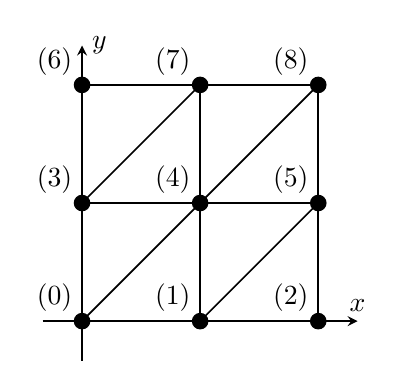
\begin{tikzpicture}
    \draw[->,>=stealth,semithick] (-0.5,0)--(3.5,0)node[above]{$x$}; %x軸
    \draw[->,>=stealth,semithick] (0,-0.5)--(0,3.5)node[right]{$y$}; %y軸\
    \draw[semithick] (3,0)--(3,3)--(0,3); 
    \draw[semithick] (1.5,0)--(1.5,3); 
    \draw[semithick] (0,1.5)--(3,1.5);
    \draw[semithick] (0,1.5)--(1.5,3);
    \draw[semithick] (0,0)--(3,3);
    \draw[semithick] (1.5,0)--(3,1.5);
    \node at (0.0,0.0)[above left] {(0)};
    \node at (1.5,0.0)[above left] {(1)};
    \node at (3.0,0.0)[above left] {(2)};
    \node at (0.0,1.5)[above left] {(3)};
    \node at (1.5,1.5)[above left] {(4)};
    \node at (3.0,1.5)[above left] {(5)};
    \node at (0.0,3.0)[above left] {(6)};
    \node at (1.5,3.0)[above left] {(7)};
    \node at (3.0,3.0)[above left] {(8)};
    \fill (0.0,0.0) circle (3pt) (1.5,0.0) circle (3pt) (3.0,0.0) circle (3pt);
    \fill (0.0,1.5) circle (3pt) (1.5,1.5) circle (3pt) (3.0,1.5) circle (3pt);
    \fill (0.0,3.0) circle (3pt) (1.5,3.0) circle (3pt) (3.0,3.0) circle (3pt);
  \end{tikzpicture}
  \caption{メッシュ分割と節点番号}
\end{figure}

要素[0],[2],[4],[6]は次の要素係数行列\(\vb*{A_{e}}\)と要素定数項ベクトル\(\vb*{f_{e}}\)を有する。
\begin{align}
  \vb{A_{e}} = \mqty(0.50 & 0.00 & -0.50 \\ 0.00 & 0.50 & -0.50 \\ -0.50 & -0.50 & 1.00)
\end{align}
\begin{align}
  \vb{f_{e}} = \mqty(-0.167 \\ -0.167 \\ -0.167)
\end{align} 
要素[1],[3],[5],[7]は次の要素係数行列\(\vb*{A_{e}}\)と要素定数項ベクトル\(\vb*{f_{e}}\)を有する。
\begin{align}
  \vb{A_{e}} = \mqty(0.500 & -0.500 & 0.00 \\ -0.500 & 1.00 & -0.500 \\ 0.000 & -0.500 & 0.500)
\end{align}
\begin{align}
  \vb{f_{e}} = \mqty(-0.167 \\ -0.167 \\ -0.167)
\end{align}

図に示された節点番号と要素番号の関係に従ってこれらを全体係数行列\(\vb*{A}\)と全体定数項ベクトル\(\vb*{f}\)に組み込む。
\begin{align}
  \vb*{A} = 
  \mqty(
     1.000 &-0.500 & 0.000 &-0.500 & 0.000 & 0.000 & 0.000 & 0.000 & 0.000 \\
    -0.500 & 2.000 &-0.500 & 0.000 &-1.000 & 0.000 & 0.000 & 0.000 & 0.000 \\
     0.000 &-0.500 & 1.000 & 0.000 & 0.000 &-0.500 & 0.000 & 0.000 & 0.000 \\
    -0.500 & 0.000 & 0.000 & 2.000 &-1.000 & 0.000 &-0.500 &  0.000 & 0.000 \\
     0.000 &-1.000 & 0.000 &-1.000 & 4.000 & -1.000 & 0.000 & -1.000 & 0.000 \\
     0.000 & 0.000 &-0.500 & 0.000 &-1.000 & 2.000 & 0.000 & 0.000 &-0.500 \\
     0.000 & 0.000 & 0.000 &-0.500 & 0.000 & 0.000 & 1.000 &-0.500 & 0.000 \\
     0.000 & 0.000 & 0.000 & 0.000 &-1.000 & 0.000 &-0.500 & 2.000 &-0.500 \\
     0.000 & 0.000 & 0.000 & 0.000 & 0.000 &-0.500 & 0.000 &-0.500 & 1.000 \\
  )
\end{align}
\begin{align}
  \vb*{f} = \mqty(-0.333 \\ -0.500 \\ -0.167 \\ -0.500 \\ -1.000 \\ -0.500 \\ -0.167 \\ -0.500 \\ -0.333)
\end{align}
ここで、節点(0),(1),(2),(3),(5),(6),(7),(8)はDirichlet境界条件によって規定されるので、これを考慮すると節点(4)における\(u=u(x)\)の近似値\(\hat{u}\)は次の様に与えられる。
\begin{align}
  A^{*}\hat{u}=f^{*}
\end{align}
ただし、
\begin{align}
  A^{*} = \vb*{A_{5,5}},
\end{align}
\begin{align}
  f^{*} = \vb*{f}[5] - \sum_{i\neq5} \vb*{A_{i,5}}\vb*{u}[5].
\end{align}
これを計算すると、\(A^{*}=4.000\)と\(f^{*}=2.000\)より、\(\hat{u}=0.500\)となる。推定誤差は0.000000e+00である。

\section{メッシュ分割と近似精度について}
前節と同様の分割の仕方で、分割数を増やしていくことを考える。各節点での誤差\(\mathrm{err}_i=\vb*{u}_i-\vb*{\hat{u}}_i\)の値の分布は表1から4の様になる。誤差分布を可視化すると図3のようになる。

\begin{table}
  \begin{center}
    \label{18m}
    \caption{18メッシュ分割における各節点の近似誤差}
    \begin{tabular}{ccc}
   \(y=2/3\) & 1.110223e-16 &-1.110223e-16 \\
   \(y=1/3\) & 0.000000e+00 & 0.000000e+00 \\
             & \(x=1/3\) & \(x=2/3\) 
    \end{tabular}
  \end{center}
\end{table}

\begin{table}
  \begin{center}
    \label{32m}
    \caption{32メッシュ分割における各節点の近似誤差}
    \begin{tabular}{cccc}
   \(y=3/4\) & 0.000000e+00 & -1.110223e-16 & 0.000000e+00 \\
   \(y=2/4\) & 0.000000e+00 & 0.000000e+00 & 0.000000e+00 \\
   \(y=1/4\) & 0.000000e+00 & 0.000000e+00 & 1.110223e-16 \\
             & \(x=1/4\) & \(x=2/4\) & \(x=3/4\) 
    \end{tabular}
  \end{center}
\end{table}

\begin{table}
  \begin{center}
    \label{50m}
    \caption{50メッシュ分割における各節点の近似誤差}
    \begin{tabular}{ccccc}
   \(y=4/5\) & 0.000000e+00 & -1.110223e-16 & -2.220446e-16 & 0.000000e+00 \\
   \(y=3/5\) &  -1.110223e-16 & -1.110223e-16 & 0.000000e+00 & 0.000000e+00 \\
   \(y=2/5\) &  -5.551115e-17 & -1.110223e-16 & 0.000000e+00 & 0.000000e+00\\
   \(y=1/5\) & -2.775558e-17 & -2.775558e-17 & 1.665335e-16 & 0.000000e+00  \\
             & \(x=1/5\) & \(x=2/5\) & \(x=3/5\) & \(x=4/5\) 
    \end{tabular}
  \end{center}
\end{table}

\begin{table}
  \begin{center}
    \label{72m}
    \caption{72メッシュ分割における各節点の近似誤差}
    \begin{tabular}{cccccc}
   \(y=5/6\) & 1.110223e-16 & -2.220446e-16 & -2.220446e-16 & -4.440892e-16 & -2.220446e-16 \\
   \(y=4/6\) & -1.110223e-16 & -1.110223e-16 & -2.220446e-16 & -4.440892e-16 & -4.440892e-16 \\
   \(y=3/6\) & -5.551115e-17 & -1.110223e-16 & -2.220446e-16 &-3.330669e-16 & -2.220446e-16 \\
   \(y=2/6\) & 0.000000e+00 & -5.551115e-17 & -5.551115e-17 & 0.000000e+00 & -1.110223e-16 \\
   \(y=1/6\) & -6.938894e-18 & 0.000000e+00 & 0.000000e+00 & 5.551115e-17 & -1.110223e-16 \\
             & \(x=1/6\) & \(x=2/6\) & \(x=3/6\) & \(x=4/6\) & \(x=5/6\) 
    \end{tabular}
  \end{center}
\end{table}

\begin{figure}[htbp]
  \label{heatmap}
  \begin{tabular}{cc}
  \begin{minipage}[b]{0.45\linewidth}
    \centering
    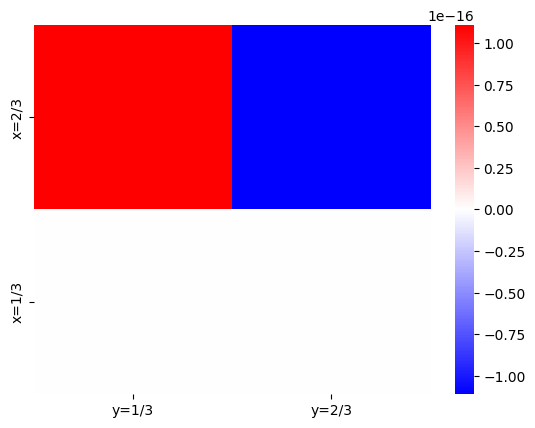
\includegraphics[keepaspectratio, scale=0.5]{img/18m.png}
    \subcaption{18meshes}
  \end{minipage} &
  \begin{minipage}[b]{0.45\linewidth}
    \centering
    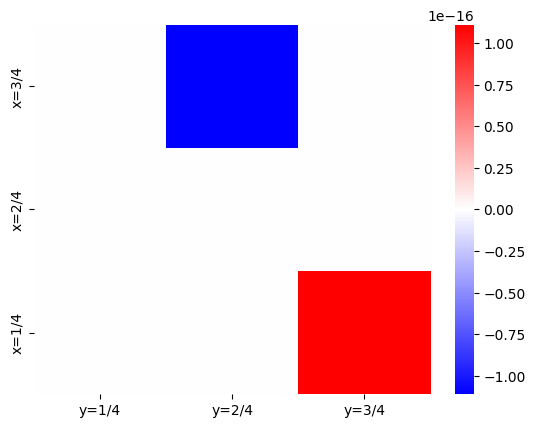
\includegraphics[keepaspectratio, scale=0.5]{img/32m.png}
    \subcaption{32meshes}
  \end{minipage} \\
  \begin{minipage}[b]{0.45\linewidth}
    \centering
    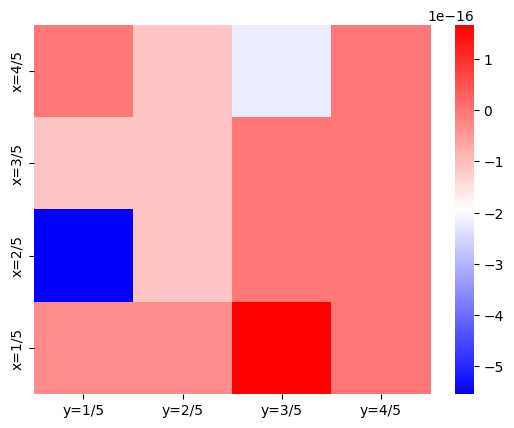
\includegraphics[keepaspectratio, scale=0.5]{img/50m.png}
    \subcaption{50meshes}
  \end{minipage} &
  \begin{minipage}[b]{0.45\linewidth}
    \centering
    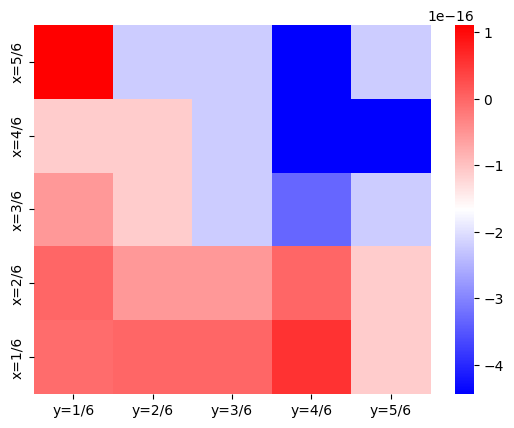
\includegraphics[keepaspectratio, scale=0.5]{img/72m.png}
    \subcaption{72meshes}
  \end{minipage}
\end{tabular}
\caption{近似誤差の分布}
\end{figure}

\begin{table}
  \begin{center}
    \label{sammry}
    \caption{まとめ}
    \begin{tabular}{cccc} \hline
      節点数 & 要素数 & (0.5,0.5)の近似値 & (0.5,0.5)の解析解との差 \\ \hline
      9 & 8 & 0.500 & 0.000 \\
      16 & 18 & 0.556 & -0.0556 \\
      25 & 32 & 0.500 & 0.000 \\
      36 & 50 & 0.520 & -0.0200 \\
      49 & 72 & 0.500 & -2.22e-16 \\ \hline
    \end{tabular}
  \end{center}
\end{table}

\end{document}